As tritium electrons are far from following the Birks's law a quenching effect is produced in the output light generated by scintillating fibers. The objective of this section is to quantify the significance of this effect and how it affects to the tritium detection.

First, a verification test of tritium electron energy deposition on scintillating fibers is carried out. In Figure \ref{fig:InitialFinalTritiumEnergy} the initial energy of tritium electrons that has reach the scintillating fibers, blue histogram, is compared with the energy deposited in scintillating fibers by them, red histogram.

\begin{figure}[h]
\centering
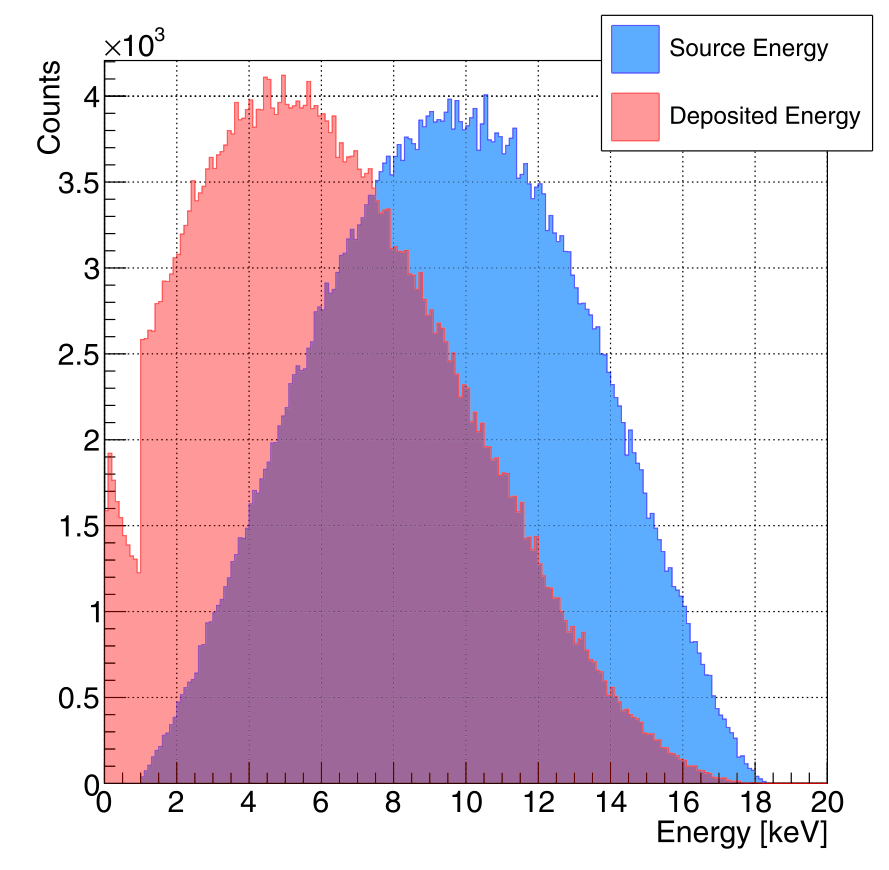
\includegraphics[scale=0.3]{8SimulationsResults/81TRITIUMDesign/812Outputlight/InitialandFinalTritiumEnergy.png}
\caption{Distribution of the initial energy of tritium events that has reach the scintillating fibers, blue histogram, and the energy deposited, red histogram.\label{fig:InitialFinalTritiumEnergy}}
\end{figure}

A shifth to the left of the spectrum (smaller energies) is observed between the blue histogram, with a peak around $10~\keV$, and the red histogram, with a peak around $5~\keV$. This displacement is mainly caused by the loss of energy from tritium electrons in the water. A cut of around $1~\keV$ is observed in both distributions. It is produced by the default energy threshold of $990~\eV$ that exist in the G4EmLivermorePhysics physics list.

Figure \ref{fig:BirksEffectinEnergyDistribution} shows two distributions of number of photons produced by tritium event, one in which the quenching effect has not been considered ($k_B=0$), red histogram, and other in which the Birks coefficient has been applied ($k_B=0.126~\mm/\MeV$), blue histogram.

\begin{figure}[h]
\centering
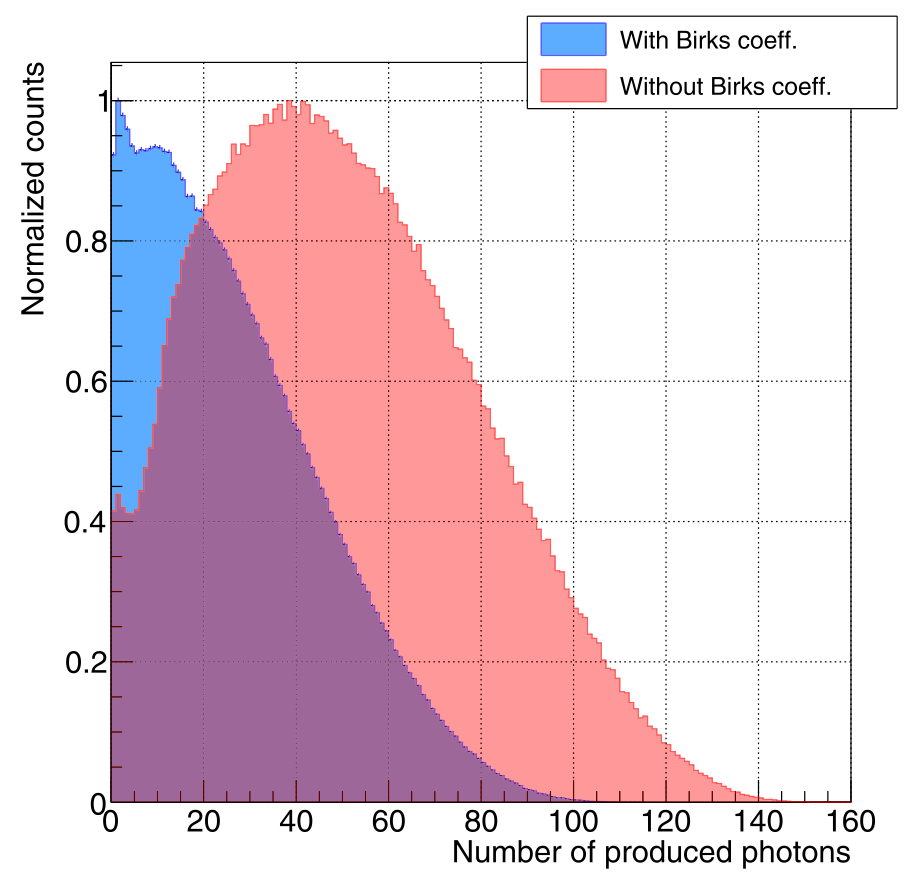
\includegraphics[scale=0.3]{8SimulationsResults/81TRITIUMDesign/812Outputlight/BirksEnergyDistribution.png}
\caption{Energy distribution of photons produced by the scintillating fiber when the birks coefficient is not considered, red histogram, and when this is considered, blue histogram.\label{fig:BirksEffectinEnergyDistribution}}
\end{figure}  

As expected, a distribution with a peak of around 40 photons per tritium event and a maximum of around 150 photons is obtained when the quenching effect was not considered. A reduction of the output light is observed when the Birks coefficient is taken into account, producing a distribution with a peak centred at $10~\keV$ and a maximum of $110~\text{Phot}$. The quenching effect is also observable in Figure \ref{fig:2DimPlotBirks}, where the number of produced photons as a function of the energy deposited in the fiber is displayed in a bidimensional plot.

\begin{figure}[h]
 \centering
  \subfloat[Quenching effect not included.]{
   \label{subfig:2DimPlotNoBirks}
    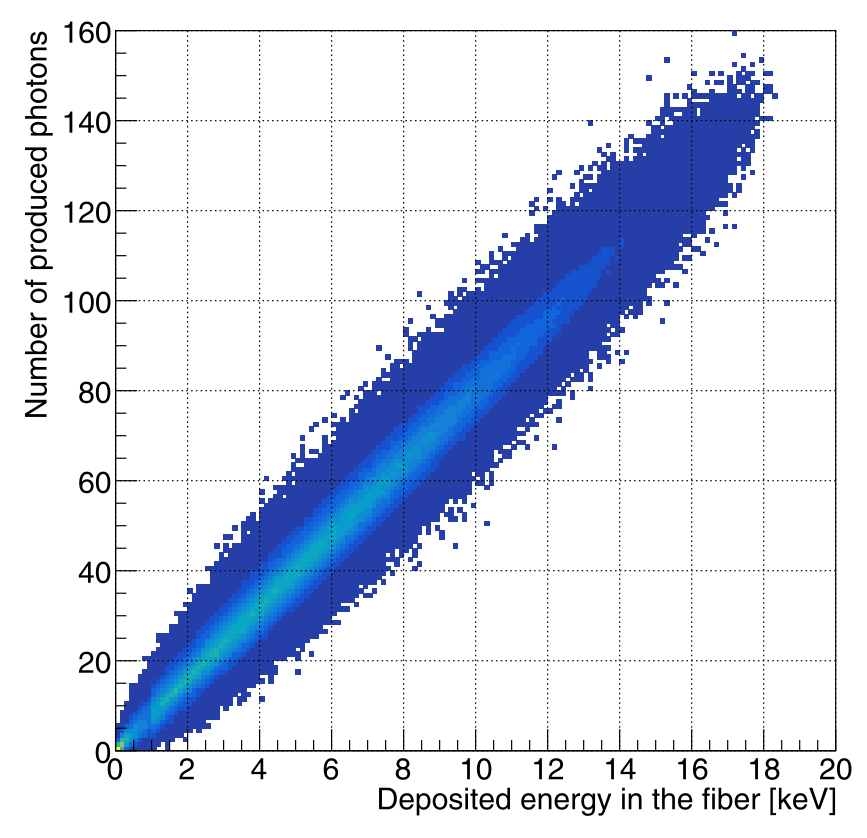
\includegraphics[width=0.4\textwidth]{8SimulationsResults/81TRITIUMDesign/812Outputlight/BidimensionalPlotBirksOFF.png}}
   %\newline
  \subfloat[Quenching effect included.]{
   \label{subfig:2DimPlotBirks}
    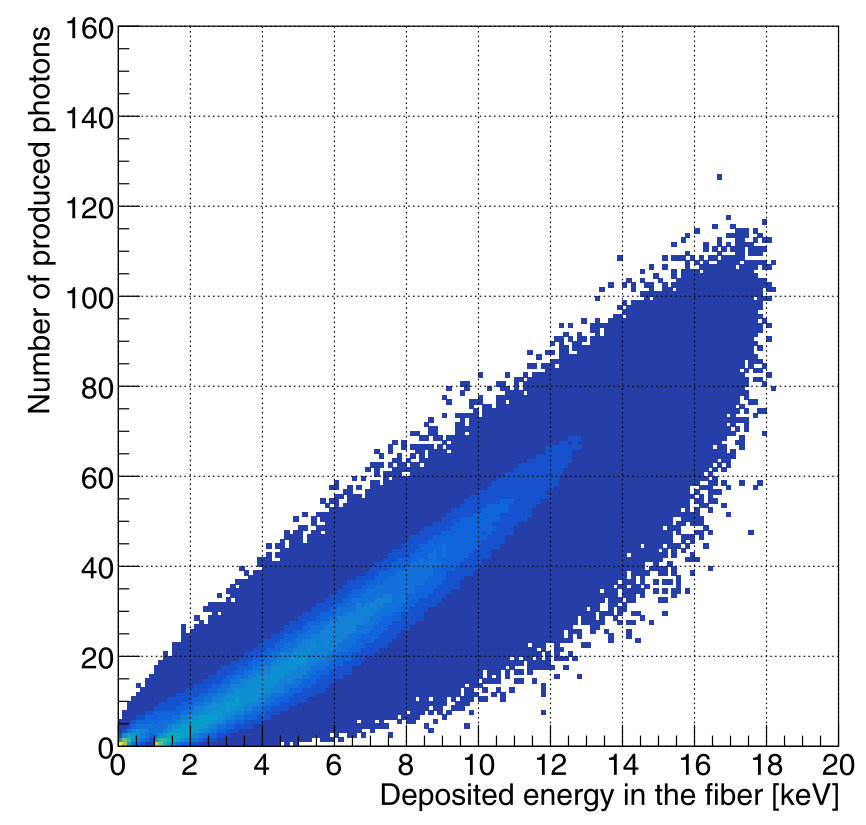
\includegraphics[width=0.4\textwidth]{8SimulationsResults/81TRITIUMDesign/812Outputlight/BidimensionalPlotBirksON.png}}
 \caption{Number of photons produced in front of the energy deposited in the scintillating fibers when a)the birks coeficient is not considered ($k_B=0$) b) the Birks coefficient is considered ($k_B=0.126~\mm/\MeV$).}
 \label{fig:2DimPlotBirks}
\end{figure}

As can be seen, since larger fluctuation in energy deposition are obtained when the birks coefficient are considered, a broader distribution is obtained.